%%%%%%%%%%%%%%%%%%%%%%%%%%%%%%%%%%%%%%%%%
% Beamer Presentation
% LaTeX Template
% Version 2.0 (March 8, 2022)
%
% This template originates from:
% https://www.LaTeXTemplates.com
%
% Author:
% Vel (vel@latextemplates.com)
%
% License:
% CC BY-NC-SA 4.0 (https://creativecommons.org/licenses/by-nc-sa/4.0/)
%
%%%%%%%%%%%%%%%%%%%%%%%%%%%%%%%%%%%%%%%%%

%----------------------------------------------------------------------------------------
%	PACKAGES AND OTHER DOCUMENT CONFIGURATIONS
%----------------------------------------------------------------------------------------

\documentclass[
11pt, % Set the default font size, options include: 8pt, 9pt, 10pt, 11pt, 12pt, 14pt, 17pt, 20pt
%t, % Uncomment to vertically align all slide content to the top of the slide, rather than the default centered
%aspectratio=169, % Uncomment to set the aspect ratio to a 16:9 ratio which matches the aspect ratio of 1080p and 4K screens and projectors
]{beamer}
\usepackage[english, russian]{babel} % выбор языка

\newcommand\rozhasize{0.20\textwidth}
\newcommand\namesize{0.18\textwidth}
\newcommand\fourpicsize{0.49\textwidth}
\usepackage{makecell}
\usepackage{tabularx}
\renewcommand{\cellalign}{vh}
\renewcommand{\theadalign}{vh}
\newcommand{\specialcell}[2][c]{%
	\begin{tabular}[#1]{@{}c@{}}#2\end{tabular}}
\graphicspath{{Images/}{./}} % Specifies where to look for included images (trailing slash required)
\definecolor{darkred}{HTML}{8b0000}
\definecolor{darkblue}{HTML}{00008B}
\usepackage{booktabs} % Allows the use of \toprule, \midrule and \bottomrule for better rules in tables
\usepackage{rotating}
\usepackage{wasysym}
\usepackage{textgreek}
\usepackage{textcomp}
%----------------------------------------------------------------------------------------
%	SELECT LAYOUT THEME
%----------------------------------------------------------------------------------------

% Beamer comes with a number of default layout themes which change the colors and layouts of slides. Below is a list of all themes available, uncomment each in turn to see what they look like.

%\usetheme{default}
%\usetheme{AnnArbor}
%\usetheme{Antibes}
%\usetheme{Bergen}
%\usetheme{Berkeley}
%\usetheme{Berlin}
%\usetheme{Boadilla}
%\usetheme{CambridgeUS}
%\usetheme{Copenhagen}
%\usetheme{Darmstadt}
%\usetheme{Dresden}
%\usetheme{Frankfurt}
%\usetheme{Goettingen}
%\usetheme{Hannover}
%\usetheme{Ilmenau}
%\usetheme{JuanLesPins}
%\usetheme{Luebeck}
%\usetheme{Madrid}
%\usetheme{Malmoe}
%\usetheme{Marburg}
%\usetheme{Montpellier}
%\usetheme{PaloAlto}
%\usetheme{Pittsburgh}
\usetheme{Rochester}
%\usetheme{Singapore}
%\usetheme{Szeged}
%\usetheme{Warsaw}

%----------------------------------------------------------------------------------------
%	SELECT COLOR THEME
%----------------------------------------------------------------------------------------

% Beamer comes with a number of color themes that can be applied to any layout theme to change its colors. Uncomment each of these in turn to see how they change the colors of your selected layout theme.

%\usecolortheme{albatross}
%\usecolortheme{beaver}
%\usecolortheme{beetle}
%\usecolortheme{crane}
%\usecolortheme{dolphin}
%\usecolortheme{dove}
%\usecolortheme{fly}
%\usecolortheme{lily}
%\usecolortheme{monarca}
%\usecolortheme{seagull}
%\usecolortheme{seahorse}
%\usecolortheme{spruce}
%\usecolortheme{whale}
%\usecolortheme{wolverine}

%----------------------------------------------------------------------------------------
%	SELECT FONT THEME & FONTS
%----------------------------------------------------------------------------------------

% Beamer comes with several font themes to easily change the fonts used in various parts of the presentation. Review the comments beside each one to decide if you would like to use it. Note that additional options can be specified for several of these font themes, consult the beamer documentation for more information.

\usefonttheme{default} % Typeset using the default sans serif font
%\usefonttheme{serif} % Typeset using the default serif font (make sure a sans font isn't being set as the default font if you use this option!)
%\usefonttheme{structurebold} % Typeset important structure text (titles, headlines, footlines, sidebar, etc) in bold
%\usefonttheme{structureitalicserif} % Typeset important structure text (titles, headlines, footlines, sidebar, etc) in italic serif
%\usefonttheme{structuresmallcapsserif} % Typeset important structure text (titles, headlines, footlines, sidebar, etc) in small caps serif

%------------------------------------------------

%\usepackage{mathptmx} % Use the Times font for serif text
\usepackage{palatino} % Use the Palatino font for serif text

%\usepackage{helvet} % Use the Helvetica font for sans serif text
\usepackage[default]{opensans} % Use the Open Sans font for sans serif text
%\usepackage[default]{FiraSans} % Use the Fira Sans font for sans serif text
%\usepackage[default]{lato} % Use the Lato font for sans serif text

%----------------------------------------------------------------------------------------
%	SELECT INNER THEME
%----------------------------------------------------------------------------------------

% Inner themes change the styling of internal slide elements, for example: bullet points, blocks, bibliography entries, title pages, theorems, etc. Uncomment each theme in turn to see what changes it makes to your presentation.

%\useinnertheme{default}
\useinnertheme{circles}
%\useinnertheme{rectangles}
%\useinnertheme{rounded}
%\useinnertheme{inmargin}

%----------------------------------------------------------------------------------------
%	SELECT OUTER THEME
%----------------------------------------------------------------------------------------

% Outer themes change the overall layout of slides, such as: header and footer lines, sidebars and slide titles. Uncomment each theme in turn to see what changes it makes to your presentation.

%\useoutertheme{default}
%\useoutertheme{infolines}
%\useoutertheme{miniframes}
%\useoutertheme{smoothbars}
%\useoutertheme{sidebar}
%\useoutertheme{split}
%\useoutertheme{shadow}
%\useoutertheme{tree}
%\useoutertheme{smoothtree}

%\setbeamertemplate{footline} % Uncomment this line to remove the footer line in all slides
%\setbeamertemplate{footline}[page number] % Uncomment this line to replace the footer line in all slides with a simple slide count

%\setbeamertemplate{navigation symbols}{} % Uncomment this line to remove the navigation symbols from the bottom of all slides

%----------------------------------------------------------------------------------------
%	PRESENTATION INFORMATION
%----------------------------------------------------------------------------------------

\title[1 к.с. Тескей-Ала-Тоо 2025]{Рассказ о горном спортивном походе 1~к.с. по Тескей-Ала-Тоо (Кырзызстан)} % The short title in the optional parameter appears at the bottom of every slide, the full title in the main parameter is only on the title page

%\subtitle{<<Делаем выводы. Или ноги>>} % Presentation subtitle, remove this command if a subtitle isn't required

\author[Остапив Лёша]{Остапив Лёша} % Presenter name(s), the optional parameter can contain a shortened version to appear on the bottom of every slide, while the main parameter will appear on the title slide

\institute[ГС МФТИ]{Горная секция МФТИ} % Your institution, the optional parameter can be used for the institution shorthand and will appear on the bottom of every slide after author names, while the required parameter is used on the title slide and can include your email address or additional information on separate lines

\date[\today]{\today} % Presentation date or conference/meeting name, the optional parameter can contain a shortened version to appear on the bottom of every slide, while the required parameter value is output to the title slide

%----------------------------------------------------------------------------------------

\begin{document}
	
	%----------------------------------------------------------------------------------------
	%	TITLE SLIDE
	%----------------------------------------------------------------------------------------
	
	\begin{frame}
		\titlepage % Output the title slide, automatically created using the text entered in the PRESENTATION INFORMATION block above
	\end{frame}
	
	%----------------------------------------------------------------------------------------
	%	TABLE OF CONTENTS SLIDE
	%----------------------------------------------------------------------------------------
	
	% The table of contents outputs the sections and subsections that appear in your presentation, specified with the standard \section and \subsection commands. You may either display all sections and subsections on one slide with \tableofcontents, or display each section at a time on subsequent slides with \tableofcontents[pausesections]. The latter is useful if you want to step through each section and mention what you will discuss.
	
	\begin{frame}
		\frametitle{Оглавление} % Slide title, remove this command for no title
		
		\tableofcontents % Output the table of contents (all sections on one slide)
		%\tableofcontents[pausesections] % Output the table of contents (break sections up across separate slides)
	\end{frame}
	
	%----------------------------------------------------------------------------------------
	%	PRESENTATION BODY SLIDES
	%----------------------------------------------------------------------------------------
	
	\section{Общая информация} % Sections are added in order to organize your presentation into discrete blocks, all sections and subsections are automatically output to the table of contents as an overview of the talk but NOT output in the presentation as separate slides
	
	%------------------------------------------------
	\subsection{Состав группы}

\begin{frame}
	\frametitle{Состав группы}
	\begin{tabular}{lllll}
	\begin{minipage}{\rozhasize}
		\includegraphics[width=\textwidth]{../pics/portraits/oa.jpg}
	\end{minipage} &
	\begin{minipage}{\rozhasize}
		\includegraphics[width=\textwidth]{../pics/portraits/dd}
	\end{minipage} &
	\begin{minipage}{\rozhasize}
		\includegraphics[width=\textwidth]{../pics/portraits/mg}
	\end{minipage} &
	\begin{minipage}{\rozhasize}
		\includegraphics[width=\textwidth]{../pics/portraits/ab}
	\end{minipage} & 
	\begin{minipage}{\namesize}
		{\tiny
		Лёша Остапив\\
		Дима Демушкин\\
		Маша Герасимова\\
		Андрей Баранов}
		\end{minipage} \\
	
	\hline
	\begin{minipage}{\rozhasize}
	\includegraphics[width=\textwidth]{../pics/portraits/ar}
	\end{minipage} &
	\begin{minipage}{\rozhasize}
		\includegraphics[width=\textwidth]{../pics/portraits/yuz}
	\end{minipage} &
	\begin{minipage}{\rozhasize}
		\includegraphics[width=\textwidth]{../pics/portraits/ak}
	\end{minipage} &
	\begin{minipage}{\rozhasize}
		\includegraphics[width=\textwidth]{../pics/portraits/in}
	\end{minipage} & 
	\begin{minipage}{\namesize}
		{\tiny
			Саша Рогозин\\
			Юля Зернина\\
			Андрей Козлов\\
			Ваня Никитин}
	\end{minipage} \\

\end{tabular}	
\end{frame}
	
	\subsection{Идея похода}
	\begin{frame}
	\frametitle{Почему Терскей?}
	\begin{itemize}
		\item Посмотреть новое с учётом пожелания и опыта группы
		\item \textit{Избежать} долгих \textit{забегов} по долинам
		\item Погулять по разному
		\item Посмотреть красивое
	\end{itemize}
	\end{frame}
	
	\subsection{Список препятствий}
	\begin{frame}
		\setbeamercovered{transparent}
		\frametitle{Список препятствий}
		\begin{enumerate}
			\item<+-> пер. Саватор, 3860) (1А)
			\item<+-> пер. Перемётный, 4026  (1А)
			\item<+-> пер. Ашутор Западный, 3700 (1А)
			\item<+-> пер. Иттиш, 3895 (1А)
			\item<+-> в. Марс, 4450 (н/к)
			\item<+-> пер. Кашкасу, 3890 (1А)
		\end{enumerate}
	\centering
	\includegraphics<1>[height=0.5\textheight]{pics/passes/savator}%
	\includegraphics<2>[height=0.5\textheight]{pics/passes/peremetnyy}%
	\includegraphics<3>[height=0.5\textheight]{pics/passes/ashutor}%
	\includegraphics<4>[height=0.5\textheight]{pics/passes/ittish}%
	\includegraphics<5>[height=0.5\textheight]{pics/passes/mars}%
	\includegraphics<5>[height=0.5\textheight]{pics/passes/kashkasuu}

	\end{frame}
	
	\subsection{Трек}
	
	\begin{frame}
		\frametitle{Трек}
		\centering
		\rotatebox{0}{
			
			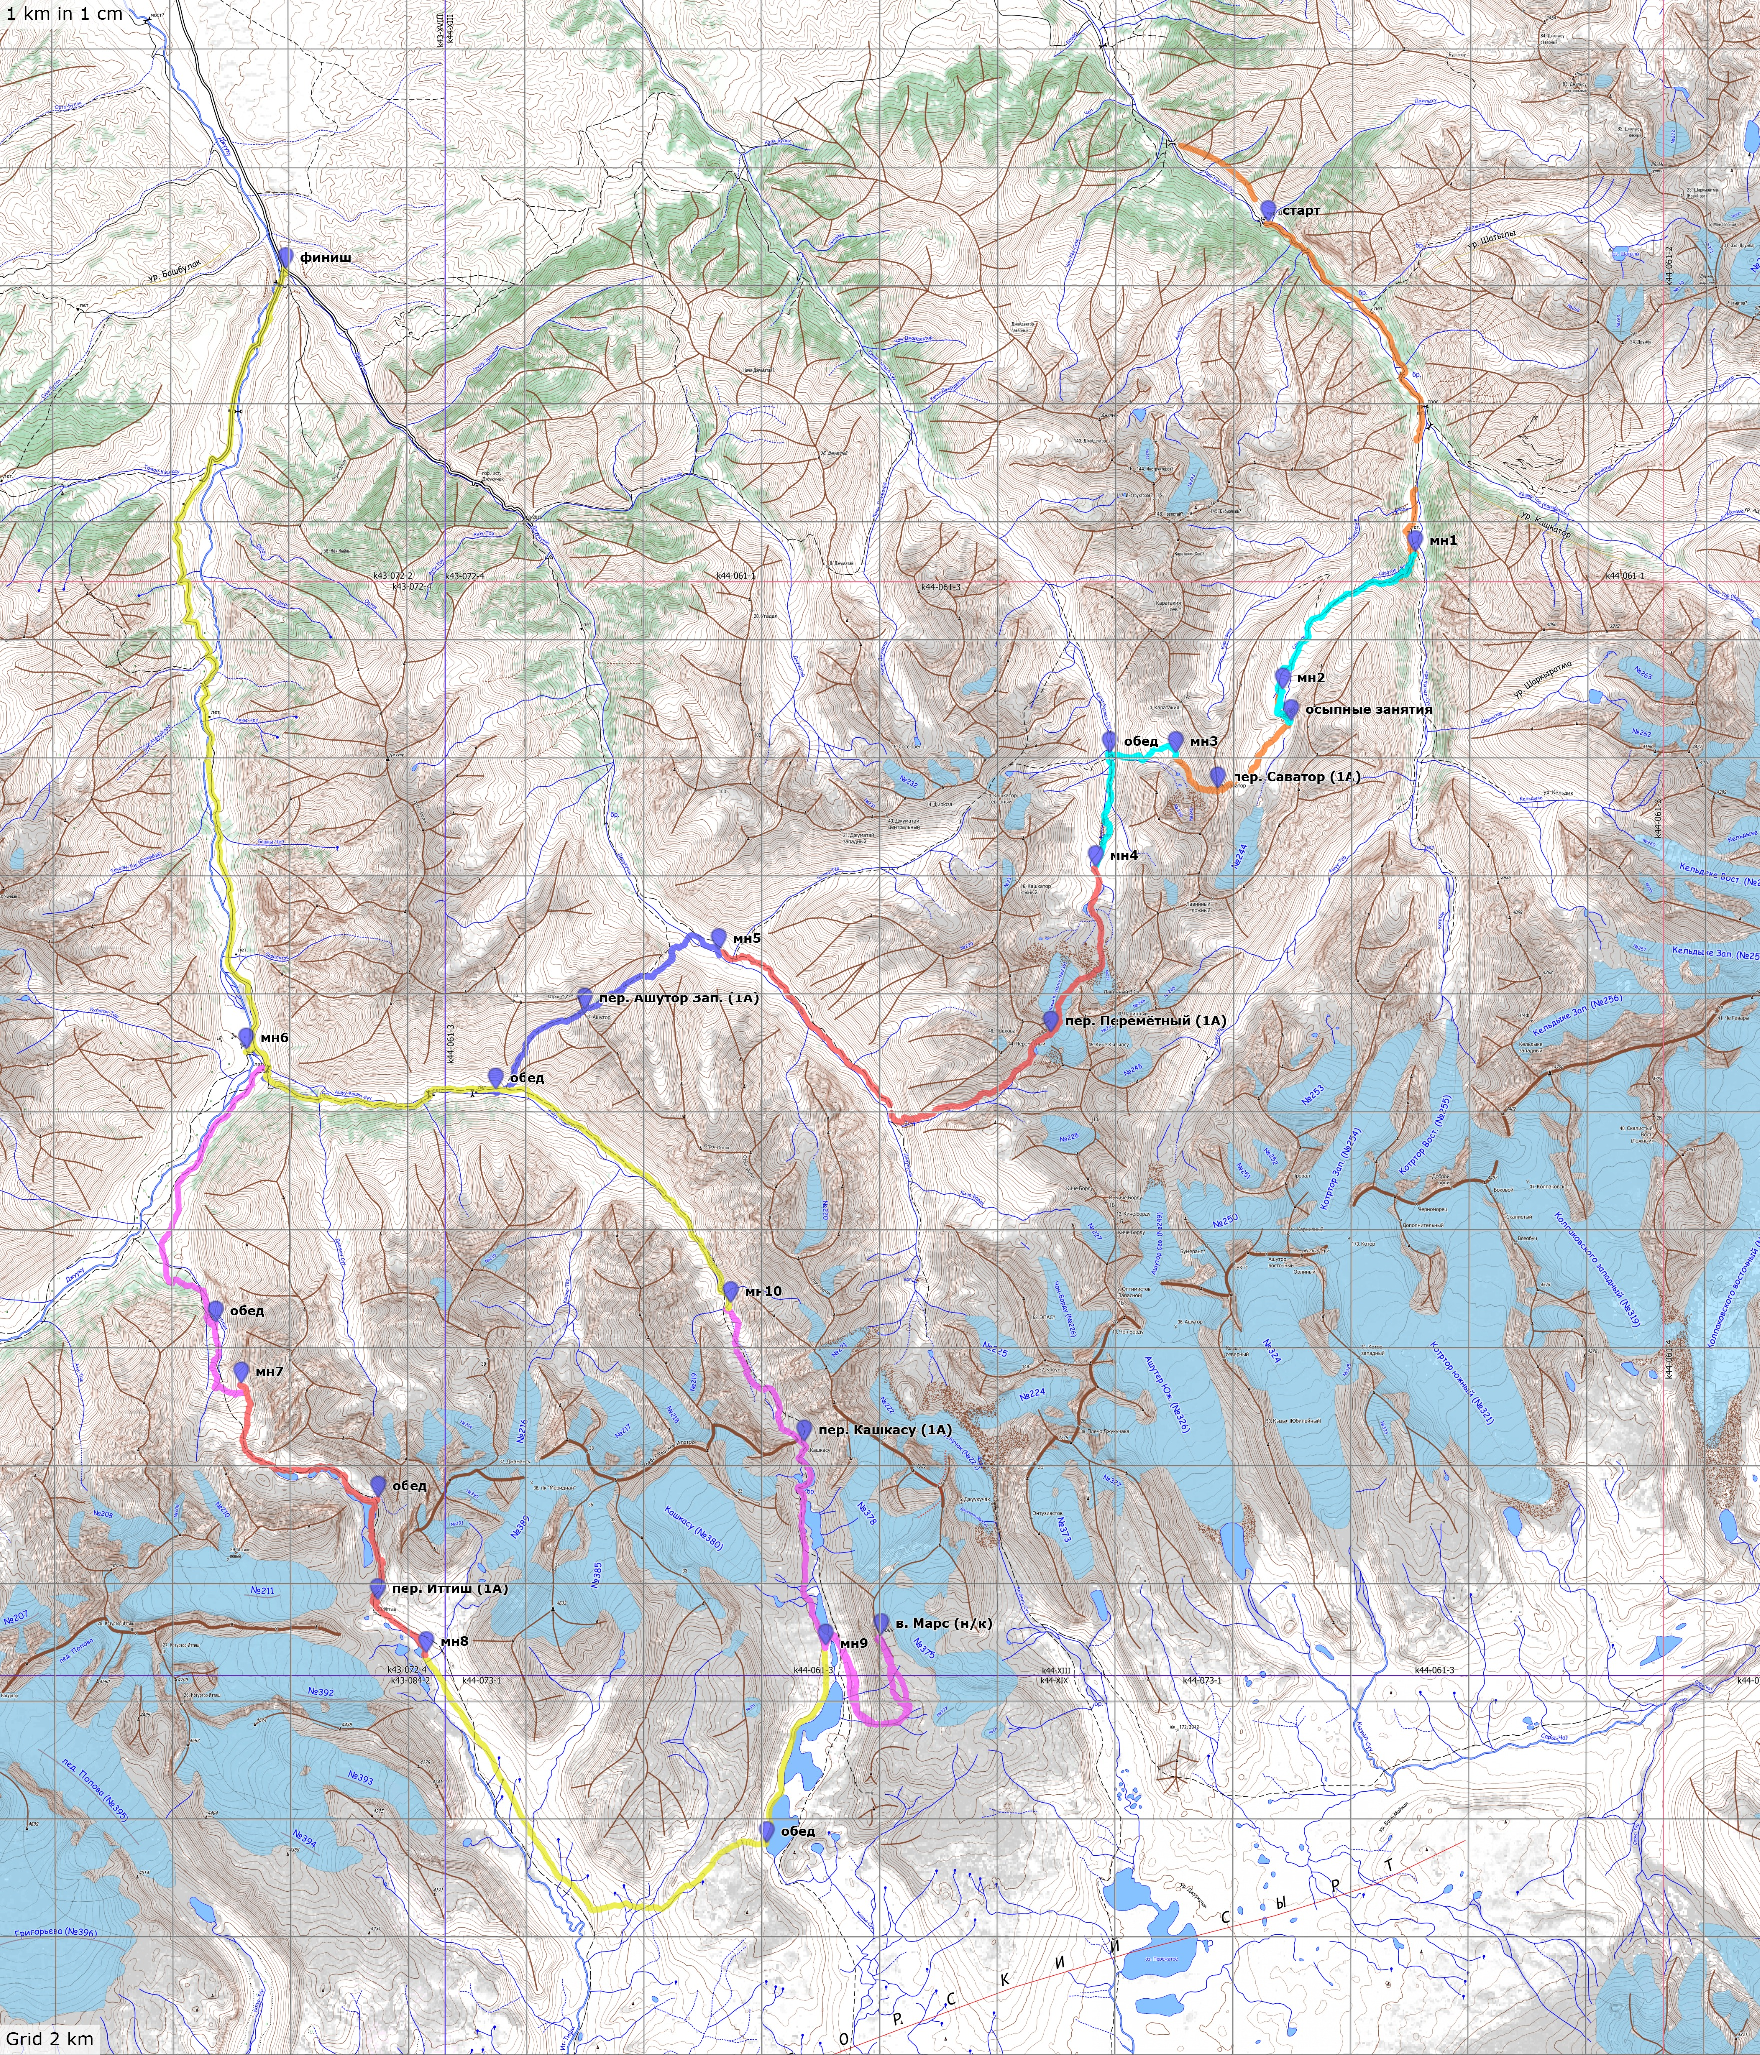
\includegraphics[width=0.6\linewidth]{../map}}		
	\end{frame}
	
	%------------------------------------------------
	\section{Отчёт по дням}
	
		\begin{frame}
	\frametitle{День 1. 03 августа}
	\framesubtitle{Старт~--- д.р. Чон-Кызыл-Суу} % Optional subtitle
	\begin{columns}[c] % The "c" option specifies centered vertical alignment while the "t" option is used for top vertical alignment
		\begin{column}{0.45\textwidth} % Left column width
			\begin{itemize}
				\item Перепаковка, старт
				\item Прошли \textbf{6.0} км
				\item ЧХВ: 03:30
				\item Набор/сброс: \textcolor{darkred}{\textbf{+550}}/\textcolor{darkblue}{\textbf{-260}}~м
			\end{itemize}
			
		\end{column}
		\begin{column}{0.5\textwidth} % Right column width
			\centering
			\includegraphics[width=\linewidth]{../pics/maps/03}
		\end{column}
	\end{columns}
\end{frame}

\begin{frame}
	\frametitle{Выход на маршрут}
	\framesubtitle{День 1, 03 августа}
	\centering
	\includegraphics[width=\linewidth]{../pics/DSC_0412}
\end{frame}



\begin{frame}
	\frametitle{д.р. Кичкинакол Уллукёльский}
	\framesubtitle{День 1, 03 августа}
	\centering
	\includegraphics[width=\linewidth]{../pics/DSC_0528}
\end{frame}

\begin{frame}
	\frametitle{Район ФГС}
	\framesubtitle{День 1, 18 августа}
	\centering
	\includegraphics[width=0.8\linewidth]{../pics/IMG_2124.jpg}
\end{frame}

\begin{frame}
	\frametitle{Реклама спальника}
	\framesubtitle{День 1, 03 августа}
	\centering
	\includegraphics[width=\linewidth]{../pics/DSC_0550}
\end{frame}

\begin{frame}
	\frametitle{д.р. Кичкинакол Уллукёльский}
	\framesubtitle{День 1, 03 августа}
	«Кичкине къол»~--- «Маленькое ущелье»
	\centering
	\includegraphics[width=\linewidth]{../pics/DSC_0558}
\end{frame}

\begin{frame}
	\frametitle{Чешем к м.н.}
	\framesubtitle{День 1, 03 августа}
	\centering
	\includegraphics[width=\linewidth]{../pics/DSC_0559}
\end{frame}

\begin{frame}
	\frametitle{д.р. Кичкинакол Уллукёльский}
	\framesubtitle{День 1, 03 августа}
	\centering
	\rotatebox{90}{\includegraphics[width=0.67\linewidth]{../pics/DSC_0563}}
\end{frame}

\begin{frame}
	\frametitle{Горечавковое}
	\framesubtitle{День 1, 03 августа}
	\centering
	\includegraphics[width=\linewidth]{../pics/DSC_0585}
\end{frame}
		\begin{frame}
	\frametitle{День 2. 04 августа}
	\framesubtitle{д.р. Саватор} % Optional subtitle
	\begin{columns}[c] % The "c" option specifies centered vertical alignment while the "t" option is used for top vertical alignment
		\begin{column}{0.45\textwidth} % Left column width
			\begin{itemize}
				\item Заполз/Забег по долине Саватора
				\item Группа Кати уходит в соседнюю долину
				\item Попытки в курумниковые занятия (не зря)
				\item Прошли \textbf{5.3} км
				\item ЧХВ: 03:45
				\item Набор/сброс: \textcolor{darkred}{\textbf{+900}}/\textcolor{darkblue}{\textbf{-105}}~м
			\end{itemize}
			
		\end{column}
		\begin{column}{0.5\textwidth} % Right column width
			\centering
			\includegraphics[width=\linewidth]{pics/maps/04}
		\end{column}
	\end{columns}
\end{frame}

\begin{frame}
	\frametitle{Подъём по д.р. Саватор}
	\framesubtitle{День 2, 04 августа}
	\centering
	\includegraphics[width=0.9\linewidth]{pics/IMG_2149.jpg}
\end{frame}


\begin{frame}
	\frametitle{Подъём по д.р. Саватор, расставание с группой Кати}
	\framesubtitle{День 2, 04 августа}
	\centering
	\includegraphics[width=\linewidth]{pics/IMG_2183.jpg}
\end{frame}

\begin{frame}
	\frametitle{Вид в обратную сторону}
	\framesubtitle{День 2, 04 августа}
	\centering
	\includegraphics[width=\linewidth]{pics/IMG_2218.jpg}
\end{frame}

\begin{frame}
	\frametitle{То же с дрона}
	\framesubtitle{День 2, 04 августа}
	\centering
	\includegraphics[width=\linewidth]{pics/drone/DJI_0038}
\end{frame}

\begin{frame}
	\frametitle{д.р. Саватор}
	\framesubtitle{День 2, 04 августа}
	\centering
	\includegraphics[width=\linewidth]{pics/IMG_2226.jpg}
\end{frame}

\begin{frame}
	\frametitle{верховья р. Саватор}
	\framesubtitle{День 2, 04 августа}
	\centering
	\includegraphics[width=\linewidth]{pics/IMG_2297.jpg}
\end{frame}
	
\begin{frame}
	\frametitle{То же с дрона}
	\framesubtitle{День 2, 04 августа}
	\centering
	\includegraphics[width=\linewidth]{pics/drone/DJI_0042}
\end{frame}
	
	\begin{frame}
	\frametitle{День 4. 05 августа}
	\framesubtitle{\textbf{пер. Саватор (1А, 3860)}} % Optional subtitle
	\begin{columns}[c] % The "c" option specifies centered vertical alignment while the "t" option is used for top vertical alignment
		\begin{column}{0.45\textwidth} % Left column width
			\begin{itemize}
				\item «Хороший, интересный, обучающий перевал»
				\item И погода приятная
				\item Прошли \textbf{5.2} км
				\item ЧХВ: 07:45
				\item Набор/сброс: \textcolor{darkred}{\textbf{+425}}/\textcolor{darkblue}{\textbf{-280}}~м
			\end{itemize}
			
		\end{column}
		\begin{column}{0.5\textwidth} % Right column width
			\centering
			\includegraphics[width=\linewidth]{pics/maps/05}
		\end{column}
	\end{columns}
\end{frame}

\begin{frame}
	\frametitle{Путь подъёма на пер. Саватор}
	\framesubtitle{День 3, 05 августа}
	\centering
	\includegraphics[width=\textwidth]{pics/IMG_2360}			
\end{frame}

\begin{frame}
	\frametitle{Бодро чешем}
	\framesubtitle{День 3, 05 августа}
	\centering
	\includegraphics[width=0.9\textwidth]{pics/IMG_2368}			
\end{frame}

\begin{frame}
	\frametitle{Подъём на пер. Саватор}
	\framesubtitle{День 3, 05 августа}
	\centering
	\includegraphics[width=0.5\textwidth]{pics/IMG_2446}			
\end{frame}

\begin{frame}
	\frametitle{Подъём на пер. Саватор}
	\framesubtitle{День 3, 05 августа}
	\centering
	\includegraphics[width=0.67\textwidth]{pics/IMG_2487}			
\end{frame}

\begin{frame}
	\frametitle{Подъём на пер. Саватор}
	\framesubtitle{День 3, 05 августа}
	
	\centering
	\includegraphics[width=0.9\textwidth]{pics/IMG_2478.jpg}			
	
\end{frame}


\begin{frame}
	\frametitle{Группа на перевале}
	\framesubtitle{День 3, 05 августа}

	\centering
	\includegraphics[width=\textwidth]{pics/IMG_2507.jpg}			
	<<Вид>> в д.р. Саватор
	
\end{frame}

\begin{frame}
	\frametitle{Группа на перевале}
	\framesubtitle{День 3, 05 августа}
	
	\centering
	\includegraphics[width=0.65\textwidth]{pics/IMG_2497.jpg}			
	
\end{frame}

\begin{frame}
	\frametitle{Группа на перевале}
	\framesubtitle{День 3, 05 августа}
	
	\centering
	\includegraphics[width=0.95\textwidth]{pics/IMG_2511.jpg}			
	<<Вид>> в д.р. Киче-Кызыл-Суу
	
\end{frame}

\begin{frame}
	\frametitle{Спускаемся с перевала}
	\framesubtitle{День 3, 05 августа}
	\centering
	\includegraphics[width=0.9\linewidth]{pics/IMG_2532.jpg}			
\end{frame}


\begin{frame}
	\frametitle{Спускаемся с перевала}
	\framesubtitle{День 3, 05 августа}
	\centering
	\includegraphics[width=0.65\linewidth]{pics/20250805_134904}			
\end{frame}


\begin{frame}
	\frametitle{Спускаемся с перевала}
	\framesubtitle{День 3, 05 августа}
	\centering
	\includegraphics[width=0.9\linewidth]{pics/IMG_2536.jpg}			
\end{frame}


\begin{frame}
	\frametitle{Спускаемся с перевала}
	\framesubtitle{День 3, 05 августа}
	\centering
	\includegraphics[width=\linewidth]{pics/IMG_2594.jpg}			
\end{frame}

\begin{frame}
	\frametitle{Потом по гребню}
	\framesubtitle{День 3, 05 августа}
	\centering
	\includegraphics[width=\linewidth]{pics/IMG_2593.jpg}			
\end{frame}

		\begin{frame}
	\frametitle{День 4. 06 августа}
	\framesubtitle{д.р. Киче-Кызыл-Суу} % Optional subtitle
	\begin{columns}[c] % The "c" option specifies centered vertical alignment while the "t" option is used for top vertical alignment
		\begin{column}{0.45\textwidth} % Left column width
			\begin{itemize}
				\item Пытаемся разглядеть Катину группу на Кашкаторе
				\item Выбираем себе перевал по вкусу
				\item Прошли \textbf{6.5} км
				\item ЧХВ: 03:15
				\item Набор/сброс: \textcolor{darkred}{\textbf{+245}}/\textcolor{darkblue}{\textbf{-305}}~м
			\end{itemize}
			
		\end{column}
		\begin{column}{0.5\textwidth} % Right column width
			\centering
			\includegraphics[width=\linewidth]{../pics/maps/06}
		\end{column}
	\end{columns}
\end{frame}



\begin{frame}
	\frametitle{Нарзанные источники}
	\framesubtitle{День 4, 06 августа}
	{\tiny
		\begin{minipage}{\fourpicsize}
			\centering
			\includegraphics[width=\textwidth]{../pics/DSC_1043}			
		\end{minipage}
		\hfill
		\begin{minipage}{\fourpicsize}
			\centering
			\includegraphics[width=0.8\textwidth]{../pics/DSC_1098}			
		\end{minipage}
		\vfill
	}
\end{frame}

\begin{frame}
	\frametitle{Учимся утилизировать использованные газовые баллоны \smiley}
	\framesubtitle{День 4, 06 августа}
	{\tiny
		\begin{minipage}{\fourpicsize}
			\centering
			\includegraphics[width=\textwidth]{../pics/DSC_1150}			
		\end{minipage}
		\hfill
		\begin{minipage}{\fourpicsize}
			\centering
			\includegraphics[width=\textwidth]{../pics/DSC_1152}			
		\end{minipage}
		\vfill
	}
\end{frame}


	
		\begin{frame}
	\frametitle{День 5. 07 августа}
	\framesubtitle{пер. Перемётный (1А, 4026)~--- д.р. Джукучак} % Optional subtitle
	\begin{columns}[c] % The "c" option specifies centered vertical alignment while the "t" option is used for top vertical alignment
		\begin{column}{0.45\textwidth} % Left column width
			\begin{itemize}
				\item Да, нам не хватило Перемётного в прошлый раз, можем повторить
				\item Прекрасный подъём
				\item Утомительный, но весёлый спуск
				\item Прошли \textbf{12.4} км
				\item ЧХВ: 10:14
				\item Набор/сброс: \textcolor{darkred}{\textbf{+465}}/\textcolor{darkblue}{\textbf{-1075}}~м
			\end{itemize}
			
		\end{column}
		\begin{column}{0.5\textwidth} % Right column width
			\centering
			\includegraphics[width=0.9\linewidth]{pics/maps/07}
		\end{column}
	\end{columns}
\end{frame}

\begin{frame}
	\frametitle{Путь подъёма по леднику}
	\framesubtitle{День 5, 07 августа}
	\centering
	\includegraphics[width=\textwidth]{pics/DJI_0059}			
\end{frame}

\begin{frame}
	\frametitle{Брод рукава Киче-Кызыл-Суу и подъём на морену}
	\framesubtitle{День 5, 07 августа}
	\centering
	\includegraphics[width=\textwidth]{pics/IMG_2778}			
\end{frame}

\begin{frame}
	\frametitle{Сеанс связи}
	\framesubtitle{День 5, 07 августа}
	\centering
	\rotatebox{-90}{\includegraphics[width=0.63\textwidth]{pics/20250807_075822}}			
\end{frame}

\begin{frame}
	\frametitle{Чешем по морене}
	\framesubtitle{День 5, 07 августа}
	\centering
	\includegraphics[width=0.9\textwidth]{pics/IMG_2825}			
\end{frame}

\begin{frame}
	\frametitle{Дошли до ледника}
	\framesubtitle{День 5, 07 августа}
	\centering
	\includegraphics[width=0.9\textwidth]{pics/IMG_2851}			
\end{frame}

\begin{frame}
	\frametitle{Чешем по леднику}
	\framesubtitle{День 5, 07 августа}
	\centering
	\includegraphics[width=0.9\textwidth]{pics/IMG_2858}			
\end{frame}

\begin{frame}
	\frametitle{Чешем по леднику}
	\framesubtitle{День 5, 07 августа}
	\centering
	\includegraphics[width=0.9\textwidth]{pics/IMG_2868}			
\end{frame}

\begin{frame}
	\frametitle{Чешем по леднику}
	\framesubtitle{День 5, 07 августа}
	\centering
	\includegraphics[width=0.9\textwidth]{pics/IMG_2880}			
\end{frame}

\begin{frame}
	\frametitle{Путь подъёма по леднику}
	\framesubtitle{День 5, 07 августа}
	\centering
	\includegraphics[width=\textwidth]{pics/view_kiche}			
\end{frame}

\begin{frame}
	\frametitle{Путь подъёма по леднику}
	\framesubtitle{День 5, 07 августа}
	\centering
	\includegraphics[width=0.9\textwidth]{pics/20250807_110046}			
\end{frame}

\begin{frame}
	\frametitle{На перевале}
	\framesubtitle{День 5, 07 августа}
	\centering
	\includegraphics[width=\textwidth]{pics/drone/DJI_0070}			
\end{frame}

\begin{frame}
	\frametitle{пер. Перемётный. Сложили тур}
	\framesubtitle{День 5, 07 августа}
	\centering
	\includegraphics[width=0.99\textwidth]{pics/typ}			
\end{frame}

\begin{frame}
	\frametitle{Путь спуска с перевала}
	\framesubtitle{День 5, 07 августа}
	\centering
	\includegraphics[width=0.9\textwidth]{pics/IMG_2970}			
\end{frame}

\begin{frame}
	\frametitle{За озером~--- галечные площадки, обед}
	\framesubtitle{День 5, 07 августа}
	\centering
	\includegraphics[width=0.9\textwidth]{pics/IMG_2994}			
\end{frame}

\begin{frame}
	\frametitle{А дальше~--- самое интересное}
	\framesubtitle{День 5, 07 августа}
	\centering
	\includegraphics[width=0.9\textwidth]{pics/IMG_3008}			
\end{frame}

\begin{frame}
	\frametitle{<<Мягкий траверс>>}
	\framesubtitle{День 5, 07 августа}
	\centering
	\includegraphics[width=0.9\textwidth]{pics/IMG_3018}			
\end{frame}

\begin{frame}
	\frametitle{Причина тряски}
	\framesubtitle{День 5, 07 августа}
	\centering
	\vspace{-0.7cm}
	\rotatebox{-90}{\includegraphics[width=0.67\textwidth]{pics/IMG_3021}}		
\end{frame}

\begin{frame}
	\frametitle{Причина тряски}
	\framesubtitle{День 5, 07 августа}
	\centering
		\rotatebox{-90}{\includegraphics[width=0.65\textwidth]{pics/20250807_133015}	}
\end{frame}

\begin{frame}
	\frametitle{}
	\framesubtitle{День 5, 07 августа}
	\centering
	\includegraphics[width=0.9\textwidth]{pics/IMG_3049}			
\end{frame}

\begin{frame}
	\frametitle{Оглядываясь назад}
	\framesubtitle{День 5, 07 августа}
	\centering
	\includegraphics[width=0.9\textwidth]{pics/IMG_3062}			
\end{frame}

\begin{frame}
	\frametitle{Спуск в долину}
	\framesubtitle{День 5, 07 августа}
	\centering
	\includegraphics[width=0.9\textwidth]{pics/IMG_3088}			
\end{frame}

\begin{frame}
	\frametitle{д.р. Джукучак}
	\framesubtitle{День 5, 07 августа}
	\centering
	\includegraphics[width=0.9\textwidth]{pics/IMG_3098}			
\end{frame}








		\begin{frame}
	\frametitle{День 6. 08 августа}
	\framesubtitle{\textbf{пер. Ашутор Западный (1А, 3411), кырг. <<Перевальное урочище>>}~--- слияние р. Ашукашкасуу и Джууку} % Optional subtitle
	\begin{columns}[c] % The "c" option specifies centered vertical alignment while the "t" option is used for top vertical alignment
		\begin{column}{0.55\textwidth} % Left column width
			\begin{itemize}
				\item А сегодня с Катиной группой встретимся?
				\item (нет)
				\item Так вот как 1А должны выглядеть!
				\item Сливаются три участника \frownie
				\item Прошли \textbf{13.8} км
				\item ЧХВ: xx:xx
				\item Набор/сброс: \textcolor{darkred}{\textbf{+710}}/\textcolor{darkblue}{\textbf{-1100}}~м
			\end{itemize}
			
		\end{column}
		\begin{column}{0.45\textwidth} % Right column width
			\centering
			\includegraphics[width=\linewidth]{pics/maps/08}
		\end{column}
	\end{columns}
\end{frame}

\begin{frame}
	\frametitle{Бродим р. Джукучак}
	\framesubtitle{День 6, 08 августа}
	\centering
	\includegraphics[width=\textwidth]{pics/f20250808_083320.jpg}			
\end{frame}

\begin{frame}
	\frametitle{Поднимаемся на перевал}
	\framesubtitle{День 6, 08 августа}
	\centering
	\includegraphics[width=0.9\textwidth]{pics/IMG_3104}			
\end{frame}

\begin{frame}
	\frametitle{}
	\framesubtitle{День 6, 08 августа}
	\centering
	\includegraphics[width=0.9\textwidth]{pics/IMG_3117}			
\end{frame}

\begin{frame}
	\frametitle{Подъём на перевал}
	\framesubtitle{День 6, 08 августа}
	\centering
	\includegraphics[width=0.9\textwidth]{pics/IMG_3126}			
\end{frame}

\begin{frame}
	\frametitle{У седловины}
	\framesubtitle{День 6, 08 августа}
	\centering
	\includegraphics[width=0.9\textwidth]{pics/IMG_3141}			
\end{frame}

\begin{frame}
	\frametitle{}
	\framesubtitle{День 6, 08 августа}
	\centering
	\includegraphics[width=0.9\textwidth]{pics/IMG_3145}			
\end{frame}

\begin{frame}
	\frametitle{На перевале Ашутор Западный}
	\framesubtitle{День 6, 08 августа}
	\centering
	\includegraphics[width=0.9\textwidth]{pics/IMG_3154}			
\end{frame}

\begin{frame}
	\frametitle{Начало спуска. Двуцветная сыпуха}
	\framesubtitle{День 6, 08 августа}
	\centering
	\includegraphics[width=0.9\textwidth]{pics/IMG_3164}			
\end{frame}

\begin{frame}
	\frametitle{Спуск. Каньон пересохшего ручья}
	\framesubtitle{День 6, 08 августа}
	\centering
	\includegraphics[width=0.9\textwidth]{pics/IMG_3167}			
\end{frame}

\begin{frame}
	\frametitle{Спуск. Каньон пересохшего ручья}
	\framesubtitle{День 6, 08 августа}
	\centering
	\includegraphics[width=0.6\textwidth]{pics/IMG_3186}			
\end{frame}

\begin{frame}
	\frametitle{д.р. Ашукашкасуу}
	\framesubtitle{День 6, 08 августа}
	\centering
	\includegraphics[width=0.9\textwidth]{pics/IMG_3210}			
\end{frame}

\begin{frame}
	\frametitle{Обедаем$\ldots$}
	\framesubtitle{День 6, 08 августа}
	\centering
	\includegraphics[width=0.9\textwidth]{pics/IMG_3223}			
\end{frame}

\begin{frame}
	\frametitle{$\ldots$обедаем$\ldots$}
	\framesubtitle{День 6, 08 августа}
	\centering
	\includegraphics[width=0.9\textwidth]{pics/IMG_3224}			
\end{frame}

\begin{frame}
	\frametitle{$\ldots$и чешем к заброске}
	\framesubtitle{День 6, 08 августа}
	\centering
	\includegraphics[width=0.9\textwidth]{pics/IMG_3233}			
\end{frame}

\begin{frame}
	\frametitle{Чешем к заброске}
	\framesubtitle{День 6, 08 августа}
	\centering
	\includegraphics[width=0.9\textwidth]{pics/IMG_3262}			
\end{frame}

\begin{frame}
	\frametitle{Жаман-Суу (кырг. <<плохая вода>>)}
	\framesubtitle{День 6, 08 августа}
	\centering
	\includegraphics[width=0.9\textwidth]{pics/IMG_3272}			
\end{frame}

\begin{frame}
	\frametitle{Слияние р. Ашукашкасуу и Джууку. Заброска}
	\framesubtitle{День 6, 08 августа}
	\centering
	\includegraphics[width=0.9\textwidth]{pics/IMG_3288}			
\end{frame}
		\begin{frame}
	\frametitle{День 7. 9 августа}
	\framesubtitle{д.р. Иттиши>	} % Optional subtitle
	\begin{columns}[c] % The "c" option specifies centered vertical alignment while the "t" option is used for top vertical alignment
		\begin{column}{0.55\textwidth} % Left column width
			\begin{itemize}
				\item Отдыхаем, перепаковываемся
				\item Чешем наверх
				\item Начинаем ловить эстетический$\ldots$ восторг от видов
				\item Прошли \textbf{9.9} км
				\item ЧХВ: 05:10
				\item Набор/сброс: \textcolor{darkred}{\textbf{+755}}/\textcolor{darkblue}{\textbf{-0}}~м
			\end{itemize}
			
		\end{column}
		\begin{column}{0.45\textwidth} % Right column width
			\centering
			\includegraphics[width=\linewidth]{../pics/maps/09}
		\end{column}
	\end{columns}
\end{frame}

\begin{frame}
	\frametitle{На спуске в д.р. Мырды}
	\framesubtitle{День 7, 09 августа}
	\centering
	\includegraphics[width=\textwidth]{../pics/DSC_0104}			
\end{frame}

		\begin{frame}
	\frametitle{День 8. 10 августа}
	\framesubtitle{\textbf{пер. Иттиш (1А, 3890)}} % Optional subtitle
	\begin{columns}[c] % The "c" option specifies centered vertical alignment while the "t" option is used for top vertical alignment
		\begin{column}{0.55\textwidth} % Left column width
			\begin{itemize}
				\item Иду вдоль озера 8 часов
				\item Жара на 3700
				\item Сырты!
				\item Встретились с группой Кати
				\item Прошли \textbf{9.5} км
				\item ЧХВ: 06:23
				\item Набор/сброс: \textcolor{darkred}{\textbf{+615}}/\textcolor{darkblue}{\textbf{-25}}~м
			\end{itemize}
			
		\end{column}
		\begin{column}{0.45\textwidth} % Right column width
			\centering
			\includegraphics[width=\linewidth]{pics/maps/10}
		\end{column}
	\end{columns}
\end{frame}



		\begin{frame}
	\frametitle{День 9. 11 августа}
	\framesubtitle{д.р. Ит-Тиши~--- сырты~--- безымянный перевал~--- озёра Кашкасу} % Optional subtitle
	\begin{columns}[c] % The "c" option specifies centered vertical alignment while the "t" option is used for top vertical alignment
		\begin{column}{0.55\textwidth} % Left column width
			\begin{itemize}
				\item Сырты, много сыртов!
				\item Офигенное озеро в обед
				\item Ветрище на м.н.
				\item Лезем на Марс завтра
				\item Прошли \textbf{12.9} км
				\item ЧХВ: 05:46
				\item Набор/сброс: \textcolor{darkred}{\textbf{+170}}/\textcolor{darkblue}{\textbf{-140}}~м
			\end{itemize}
			
		\end{column}
		\begin{column}{0.45\textwidth} % Right column width
			\centering
			\includegraphics[width=\linewidth]{../pics/maps/11}
		\end{column}
	\end{columns}
\end{frame}

\begin{frame}
	\frametitle{Утро}
	\framesubtitle{День 9, 11 августа}
	\centering
	\includegraphics[width=\textwidth]{../pics/DSC_0190}			
\end{frame}



\begin{frame}
	\frametitle{Группа на пер. Кичкинекол Малый (1А)}
	\framesubtitle{День 9, 26 августа}
	{\tiny
		\begin{minipage}{\fourpicsize}
			\centering
			\includegraphics[width=\textwidth]{../pics/DSC_0239}			
			Вид в д.р. Чунгур-Джар
		\end{minipage}
		\hfill
		\begin{minipage}{\fourpicsize}
			\centering
			\includegraphics[width=\textwidth]{../pics/DSC_0242}			
			Вид в д.р. Таллычат
		\end{minipage}
		\vfill
	}
\end{frame}
		\begin{frame}
	\frametitle{День 10. 12 августа}
	\framesubtitle{\textbf{в. Марс (н/к, 4450)}~---\textbf{пер. Кашкасу (1А, 3890)}~--- д.р. Танышхан} % Optional subtitle
	\begin{columns}[c] % The "c" option specifies centered vertical alignment while the "t" option is used for top vertical alignment
		\begin{column}{0.55\textwidth} % Left column width
			\begin{itemize}
				\item С утра пораньше смотались на Марс (и обратно)
				\item Вайбовейший пер. Кашкасу
				\item И снова эстетический восторг
				\item Прошли \textbf{13.1} км
				\item ЧХВ: 07:48
				\item Набор/сброс: \textcolor{darkred}{\textbf{+439}}/\textcolor{darkblue}{\textbf{-1024}}~м
			\end{itemize}
			
		\end{column}
		\begin{column}{0.45\textwidth} % Right column width
			\centering
			\includegraphics[width=\linewidth]{pics/maps/12}
		\end{column}
	\end{columns}
\end{frame}

\begin{frame}
	\frametitle{Начало подъёма}
	\framesubtitle{День 10, 12 августа}
	\centering
	\includegraphics[width=0.9\linewidth]{pics/IMG_3565.jpg}			
\end{frame}

\begin{frame}
	\frametitle{Ползём по склону}
	\framesubtitle{День 10, 12 августа}
	\centering
	\includegraphics[width=0.9\linewidth]{pics/IMG_3569.jpg}	
\end{frame}

\begin{frame}
	\frametitle{В амфитеатре}
	\framesubtitle{День 10, 12 августа}
	\centering
	\includegraphics[width=0.9\linewidth]{pics/IMG_3570.jpg}	
\end{frame}

\begin{frame}
	\frametitle{На предвершинном плато}
	\framesubtitle{День 10, 12 августа}
	\centering
	\includegraphics[width=0.9\linewidth]{pics/IMG_3576.jpg}	
\end{frame}

\begin{frame}
	\frametitle{Гладкие камушки}
	\framesubtitle{День 10, 12 августа}
	\centering
	\includegraphics[width=0.9\linewidth]{pics/IMG_3577.jpg}	
\end{frame}

\begin{frame}
	\frametitle{Ак-шийрак}
	\framesubtitle{День 10, 12 августа}
	\centering
	\includegraphics[width=0.9\linewidth]{pics/IMG_3581.jpg}	
\end{frame}

\begin{frame}
	\frametitle{Вид с вершины на Акшийрак}
	\framesubtitle{День 10, 12 августа}
	\centering
	\includegraphics[width=0.99\linewidth]{pics/IMG_3584.jpg}			
\end{frame}

\begin{frame}
	\frametitle{Ето мы}
	\framesubtitle{День 10, 12 августа}
	\centering
	\includegraphics[width=0.9\linewidth]{pics/IMG_3590.jpg}			
\end{frame}

\begin{frame}
	\frametitle{Вид с вершины на д.р. Кашкасу (на север)}
	\framesubtitle{День 10, 12 августа}
	\centering
	\includegraphics[width=0.9\linewidth]{pics/IMG_3598.jpg}			
\end{frame}

\begin{frame}
	\frametitle{в. Марс}
	\framesubtitle{День 10, 12 августа}
	\centering
	\includegraphics[width=0.9\linewidth]{pics/IMG_3600.jpg}			
\end{frame}

\begin{frame}
	\frametitle{Движение в сторону перевала от м.н.}
	\framesubtitle{День 10, 12 августа}
	\centering
	\includegraphics[width=\textwidth]{pics/20250812_110552.jpg}			
\end{frame}

\begin{frame}
	\frametitle{Где-то там перевал. Река течет туда же}
	\framesubtitle{День 10, 12 августа}
	\centering
	\includegraphics[width=0.9\textwidth]{pics/IMG_3616}			
\end{frame}

\begin{frame}
	\frametitle{Ну за этим поворотом точно перевал будет}
	\framesubtitle{День 10, 12 августа}
	\centering
	\includegraphics[width=0.55\textwidth]{pics/IMG_3620}			
\end{frame}

\begin{frame}
	\frametitle{Атмосферное тут место}
	\framesubtitle{День 10, 12 августа}
	\centering
	\includegraphics[width=0.55\textwidth]{pics/20250812_122606.jpg}	
\end{frame}

\begin{frame}
	\frametitle{Вид на юг. Река уходит под камни}
	\framesubtitle{День 10, 12 августа}
	\centering
	\includegraphics[width=0.9\textwidth]{pics/IMG_3623}			
\end{frame}

\begin{frame}
	\frametitle{пер. Кашкасу, вид в д.р. Ашукашкасу}
	\framesubtitle{День 10, 12 августа}
	\centering
	\includegraphics[width=\textwidth]{pics/IMG_3624}	
\end{frame}

\begin{frame}
	\frametitle{пер. Кашкасу, вид в д.р. Кашкасу}
	\framesubtitle{День 10, 12 августа}
	\centering
	\includegraphics[width=\textwidth]{pics/IMG_3626}	
\end{frame}

\begin{frame}
	\frametitle{По левому борту вот такое дают}
	\framesubtitle{День 10, 12 августа}
	\centering
	\includegraphics[width=0.9\textwidth]{pics/IMG_3628}			
\end{frame}

\begin{frame}
	\frametitle{И такое}
	\framesubtitle{День 10, 12 августа}
	\centering
	\includegraphics[width=0.9\textwidth]{pics/IMG_3634}			
\end{frame}

\begin{frame}
	\frametitle{И даже такое}
	\framesubtitle{День 10, 12 августа}
	\centering
	\includegraphics[width=0.9\textwidth]{pics/IMG_3639}			
\end{frame}

\begin{frame}
	\frametitle{Начало спуска с перевала}
	\framesubtitle{День 10, 12 августа}
	\centering
	\includegraphics[width=\textwidth]{pics/20250812_144637.jpg}	
\end{frame}

\begin{frame}
	\frametitle{Идем по гребням (Ковинов негодуе)}
	\framesubtitle{День 10, 12 августа}
	\centering
	\includegraphics[width=0.9\textwidth]{pics/IMG_3636}			
\end{frame}

\begin{frame}
	\frametitle{Группа Кати на обеде. наше м.н.}
	\framesubtitle{День 10, 12 августа}
	\centering
	\includegraphics[width=0.9\textwidth]{pics/IMG_3641}			
\end{frame}


	\begin{frame}
	\frametitle{День 11. 13 августа}
	\framesubtitle{д.р. Ашукашкасуу~--- д.р. Джууку~--- слияние р. Джууку и Джукучак (Финиш)} % Optional subtitle
	\begin{columns}[c] % The "c" option specifies centered vertical alignment while the "t" option is used for top vertical alignment
		\begin{column}{0.55\textwidth} % Left column width
			\begin{itemize}
				\item Четверо сходят
				\item Солнышко светит
				\item А в среднегорье, оказывается, красиво
				\item Прошли \textbf{26.1} км
				\item ЧХВ: 06:47
				\item Набор/сброс: \textcolor{darkred}{\textbf{+0}}/\textcolor{darkblue}{\textbf{-1310}}~м
			\end{itemize}			
		\end{column}
		\begin{column}{0.45\textwidth} % Right column width
			\centering
			\includegraphics[width=\linewidth]{../pics/maps/13}
		\end{column}
	\end{columns}
\end{frame}



\begin{frame}
	\frametitle{Начало спуска с м.н.}
	\framesubtitle{День 11, 13 августа}	
	\centering
	\includegraphics[width=\textwidth]{../pics/20250813_090014.jpg}			
\end{frame}

\begin{frame}
	\frametitle{Верховья р. Ашукашкасуу, последние древние морены}
	\framesubtitle{День 11, 13 августа}	
	\centering
	\includegraphics[width=0.95\textwidth]{pics/IMG_3646.jpg}			
\end{frame}

\begin{frame}
	\frametitle{д.р. Ашукашкасуу}
	\framesubtitle{День 11, 13 августа}
	\centering
	\includegraphics[width=\textwidth]{pics/IMG_3649}	
\end{frame}


\begin{frame}
	\frametitle{Забег по д.р. Джууку}
	\framesubtitle{День 11, 13 августа}		
	\centering
	\includegraphics[width=\textwidth]{pics/20250813_150637.jpg}	
\end{frame}

\begin{frame}
	\frametitle{Забег по д.р. Джууку}
	\framesubtitle{День 11, 13 августа}		
	\centering
	\includegraphics[width=\textwidth]{pics/20250813_160451.jpg}	
\end{frame}

\begin{frame}
	\frametitle{Слияние р. Джууку и Джукучак, финиш}
	\framesubtitle{День 11, 13 августа}		
	\centering
	\includegraphics[width=\textwidth]{pics/finish}	
\end{frame}

	\begin{frame}
	\frametitle{Дни 12--13. 14--15 августа}
	\framesubtitle{Послепоходовое} % Optional subtitle
	\begin{columns}[c] % The "c" option specifies centered vertical alignment while the "t" option is used for top vertical alignment
		\begin{column}{0.55\textwidth} % Left column width
			\begin{itemize}
				\item Чилл на Иссык-Куле
				\item Каньон <<Сказка>>
			\end{itemize}			
		\end{column}
		\begin{column}{0.45\textwidth} % Right column width
			\centering
			\includegraphics[width=\linewidth]{pics/maps/14_15}
		\end{column}
	\end{columns}
\end{frame}

\begin{frame}
	\frametitle{Каньон <<Сказка>>}
	\framesubtitle{Дни 12--13. 14--15 августа}	
	\centering
	\includegraphics[width=\textwidth]{pics/20250815_201423}		
\end{frame}


\begin{frame}
	\frametitle{Каньон <<Сказка>>}
	\framesubtitle{Дни 12--13. 14--15 августа}	
	\centering
	\includegraphics[width=\textwidth]{pics/20250815_100457}		
\end{frame}


\begin{frame}
	\frametitle{Каньон <<Сказка>>}
	\framesubtitle{Дни 12--13. 14--15 августа}	
	\centering
	\includegraphics[width=\textwidth]{pics/20250815_100503}			
\end{frame}

	\section{Итоги похода, выводы и рекомендации по совершённому походу (от лица руководителя)}

\subsection{Выбор и прохождение маршрута}  
\begin{enumerate}
	\item Главное: по моему мнению, на Тескей-Ала-Тоо можно и нужно проводить горные <<единички>>. Этому способствует относительно простая логистика, разнообразие рельефа и опция пересечь главный хребет (в вашем распоряжении три недалеко отстоящих друг от друга перевалов 1А). Также <<изюминкой>> похода может быть обзорная точка района~--- вершина Марс. Однако стоит иметь в виду б\'{о}льшие, чем на Кавказе, высоты и более сложную, чем на Кавказе, логистику. Поэтому идеальным мне кажется вариант, в котором участники похода уже имеют горный или высотный опыт и хотя бы частично схожены, поскольку в ситуации, если что-то пойдёт не так, решать проблемы будет заметно сложнее, чем на Кавказе.
	\item Намеренно низкий темп движения (для этого ставили одним из первых самого неторопливого участника) в первые, в том числе перевальные, дни, по моему мнению, способствовал более хорошему общему самочувствию группы и более плавной акклиматизации. Оцениваю процесс акклиматизации в этом походе как более удачный и плавный по сравнению с прошлогодним походом по Гвандре \cite{Snegovskaya2024}. Общий тайминг дня также был удачным, время выхода было таким, что мы с нашим неспешным темпом вставали на бивак в среднем за несколько часов до заката и ни разу не ходили в темное время суток;
	\item Решение включить перевалы Саватор и Перемётный в нитку было не до конца моим, а возникло в силу необходимости частично <<развести>> нитку маршрута с Катиной. Эти перевалы явно сложнее среднестатистических 1А, и то, что они стояли первыми, не совсем хорошо. Тем не менее, для группы с уровнем физической и технической подготовки средний и выше, прохождение этих перевалов, в том числе и первыми, категорически рекомендую. Они разнообразны, интересны и малохожены, а на пер. Перемётный предоставляется замечательная возможность походить по пологому леднику в <<единичке>>; 
	\item Хоть ледник из предыдущего похода и пологий, несколько пар кошек на группу взять всё-таки ст\'{о}ит;
	\item Вершина Марс горячо рекомендуется к посещению. Несмотря на то, кто, кажется, виды с неё красивее во второй половине дня, рекомендую не рисковать и заходить на неё с утра;
	\item При планировании маршрута пятнадцатикилометровый забег по грунтовке от слияния р. Ашукашкасуу и Джууку до слияния р. Джууку и Джукучак казался мне скучным мероприятием для выполнения норматива. Но на месте я, и, как минимум, некоторые участники, были в восторге от красивых видов: красных скал, поросших густым зеленым кустарником. Здесь определённо стоит пройти и насладиться видами, чтобы глаз уставший от многодневних осыпей, отдохнул на более близкой к человеку природе.
	
\end{enumerate}


\subsection{Подготовка к походу и взаимодействие с группой} 
	\begin{enumerate}
		\item С технической стороны лимитирующими скорость группы факторами было неумение некоторых участников ходить по средней осыпи и осуществлять страховку альпенштоком~--- обычная история для новичковых походов. Поэтому следует по возможности и наличию места тренировки отрабатывать эти навыки заранее. Мы это делали весной в Приэльбрусье \cite{ostapiv2025}, и это подняло средний уровень альпенштокования в группе \smiley; 
		\item Уровень взаимодействия с группой на маршруте по вопросам стратегии и тактике  оцениваю, как минимум, как достаточный (или выше). Дело в том, что в прошлом походе по Гвандре \cite{Snegovskaya2024} недостаточность такого общения была для нескольних участников важной проблемой.
		
		 
		\item Так вышло, что с группой Кати шли раздельно (сначала~-- из-за нашего отставания на спуске с пер. Саватор, а после пер. Иттиш, фактически, намеренно, посколько наши группы уже стали достаточно самодостаточны, чтобы двигаться самостоятельно). Это скорее хорошо, чем плохо, так как управлять одной группой сложнее, да и внутри каждой из групп народ друг к другу <<притёрся>>, что привело к радикально разным уровням коммуникации в группах. Катина группа была значительно более активной и разговорчивой, в то время как мы были более спокойны и менее разговорчивы. Как следствие, объединение групп после пер. Иттиш было для нашей группы серьёзным испытанием, после чего мы всё-таки пошли раздельными группами;
		\item Возможно, в силу небольшого состава в группе поддерживался очень хороший психологический климат~--- лучший за все 4 предыдущих похода руководителя. Большая благодарность участникам за усилия, прилагаемые к этому \smiley
	\end{enumerate} 
	

	\clearpage
	
	\section{Выводы}
	
	%------------------------------------------------
	
	\begin{frame}[plain] % The optional argument 'plain' hides the headline and footline
		\begin{center}
			{\Huge The End}
			
			\bigskip\bigskip % Vertical whitespace
			
			{\LARGE Questions? Comments?}
		\end{center}
	\end{frame}
	
	%----------------------------------------------------------------------------------------
	
\end{document} 